\chapter{Results}
\label{Results}

In this chapter, we describe the experiments conducted, beginning with the experimental setup and technology settings used (Section \ref{sec:setup}). We then compare the heuristic with the exact model using a fixed $T$ (obtained by the heuristic) (Section \ref{sec:comparison}), and finally, we present the phase transition in the heuristic, normalizing by individual drone paths (Section \ref{sec:transition}). This approach allows us to illustrate the advantages and limitations of our method.

All experiments were performed on a 64-bit operating system with an Intel(R) Core(TM) i7-7700 CPU @ 3.60GHz and 16GB of RAM.

\section{Experimental Setup and Technologies}
\label{sec:setup}

All experiments were conducted using the following software and tools:

\subsection{Heuristic Implementation in C\texttt{++}}

The heuristic approach was implemented in C\texttt{++}, chosen for its efficiency and control over system resources. Key components include:

\begin{itemize}
\item \textbf{Standard Library Containers}: The heuristic utilized standard C\texttt{++} library containers such as \texttt{vector} and \texttt{map} for efficient data management and manipulation. 
\item \textbf{Version and Compiler}: The implementation made use of C\texttt{++}20, and the code was compiled using the GNU GCC compiler.
\end{itemize}

\subsection{Exact Model Implementation in Julia}

The exact model was implemented in Julia, chosen for its high-performance capabilities and ease of use in mathematical and scientific computing. Key aspects include:

\begin{itemize}
\item \textbf{JuMP Package}: The exact model's optimization tasks were carried out using the \texttt{JuMP} package \cite{JuMPLubin2023}, a domain-specific modeling language for mathematical optimization embedded in Julia.
\item \textbf{Gurobi Solver}: Gurobi was used as the Mixed-Integer Linear Programming (MILP) solver, interfaced through Julia, to solve the optimization problems with high precision and performance.
\end{itemize}

\subsection{Experimentation and Analysis}

The comparison, experiments, and plots were conducted in Julia. The workflow included the following steps:

\begin{itemize}
\item \textbf{Calling C\texttt{++} Heuristic}: The compiled C\texttt{++} heuristic code was called externally from Julia. Input data was passed as files to the C\texttt{++} program.
\item \textbf{Data Handling}: The output from the C\texttt{++} heuristic was read back into Julia for further analysis.
\item \textbf{Visualization}: Results were plotted using the \texttt{Plots.jl} package in Julia.
\end{itemize}

\subsection{Drone Generation}

The experimental setup involved generating random samples for the drones' initial and final positions, varying the number of drones and the size of the grid. For each drone $k \in \{1, \ldots, K\}$, where $K$ is the current number of drones, the starting position $(x_k^{\text{start}}, y_k^{\text{start}})$ and ending position $(x_k^{\text{end}}, y_k^{\text{end}})$ were randomly selected within a grid of size $N \times M$, where $N$ and $M$ are the dimensions of the grid.

Formally, for each number of drones $K \in \{1, \ldots, R\}$, where $R$ is the maximum number of drones, and for each sample/trial $s \in \{1, \ldots, S\}$, the following procedure was applied:

\begin{itemize}
\item \textbf{Drone Generation}: For each drone $k \in \{1, \ldots, K\}$:
  \begin{itemize}
  \item Randomly generate $(x_k^{\text{start}}, y_k^{\text{start}}) \in \{1, \ldots, N\} \times \{1, \ldots, M\}$
  \item Randomly generate $(x_k^{\text{end}}, y_k^{\text{end}}) \in \{1, \ldots, N\} \times \{1, \ldots, M\}$, ensuring $(x_k^{\text{end}}, y_k^{\text{end}}) \neq (x_k^{\text{start}}, y_k^{\text{start}})$
  \end{itemize}
\end{itemize}

\section{Models Comparison}
\label{sec:comparison}

In this section, we compare the two models in terms of optimality(objective performance) and computational efficiency(running time). The x-axis in each plot represents the number of drones used to generate 20 samples per number of drones in the box plots, conducted in a 5x5 grid. The input $T$ for the exact model in each sample is the one returned by the heuristic, that is, $ T_{\text{exact\_model}} \vcentcolon  = T_{\text{heuristic}}$.

\subsection{Objective Function Performance}

We first evaluate the performance of both models in terms of their objective function outcomes. The objective function (y-axis) represents the optimization goal of minimizing path lengths for drones while avoiding collisions. Figure \ref{fig:exact_model_obj} and Figure \ref{fig:heuristic_obj} depict box plots comparing the objective function values achieved by the exact model and the heuristic model, respectively. 

Figure \ref{fig:exact_model_obj} presents the distribution of objective function values obtained by the exact model, illustrating the spread and central tendency of the outcomes across different scenarios. Conversely, Figure \ref{fig:heuristic_obj} showcases the corresponding results for the heuristic model. By comparing these plots, we can gain valuable insights into the performance of each model in optimizing the objective function.

In the scenario where $n_{\text{drones}} = 1$, the heuristic model performs as optimally as the exact model since the BFS guarantees optimality in this simple case. However, as the number of drones increases, the performance of the heuristic model diminishes. This decline in performance is anticipated due to the increased traffic within a fixed grid size, leading to more complex interactions and potential conflicts between the drones.


\begin{figure}[H]
    \centering
    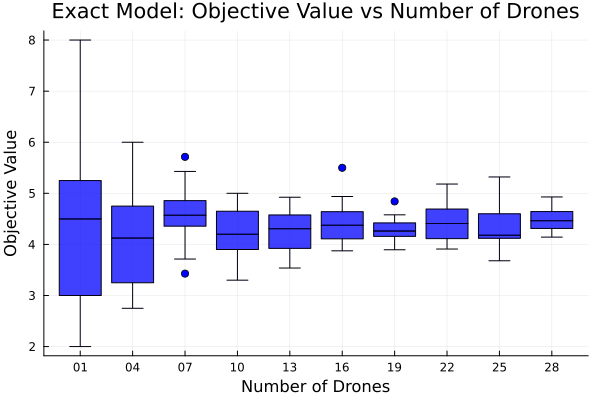
\includegraphics[width=0.8\textwidth]{img/julia_obj_boxplot_vs_drones.png}
    \caption{Exact Model Objective. Source: The authors.}
    \label{fig:exact_model_obj}
\end{figure}

\begin{figure}[H]
    \centering
    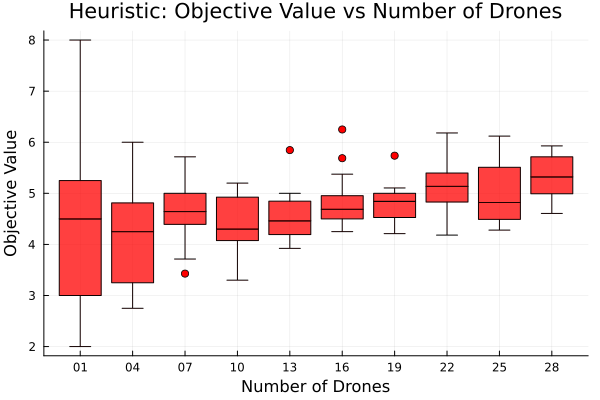
\includegraphics[width=0.8\textwidth]{img/cpp_obj_boxplot_vs_drones.png}
    \caption{Heuristic Objective. Source: The authors.}
    \label{fig:heuristic_obj}
\end{figure}


\subsection{Computational Efficiency}

Next, we analyze the computational efficiency of the two models, focusing on the time required (y-axis) to compute the optimal paths for drones. Figures \ref{fig:exact_model_time} and \ref{fig:heuristic_time} display box plots representing the computational time taken by the exact model and the heuristic model, respectively. 

Figure \ref{fig:exact_model_time} illustrates the distribution of computational times for the exact model. This plot provides an understanding of the computational overhead associated with solving the optimization problem precisely. Conversely, Figure \ref{fig:heuristic_time} presents the computational times required by the heuristic model. By comparing these plots, we assess the trade-off between computational efficiency and solution optimality offered by each model.

As illustrated in Figure \ref{fig:exact_model_time}, the heuristic consistently exhibits a lower running time compared to the exact model. This disparity in running times is not merely a constant difference but reflects the inherent differences in computational complexity between the two approaches. The heuristic model demonstrates an almost constant running time, attributed to its sub-linear performance relative to the number of drones, as discussed in Section \ref{secc:complexity_analysis}. In contrast, the exact model, being NP-complete, has constraints that cause its performance to depend exponentially on both the number of drones and the specified $T$. Consequently, the running time of the exact model increases exponentially with the number of drones, as evidenced by the plot in Figure \ref{fig:exact_model_time}.


\begin{figure}[H]
    \centering
    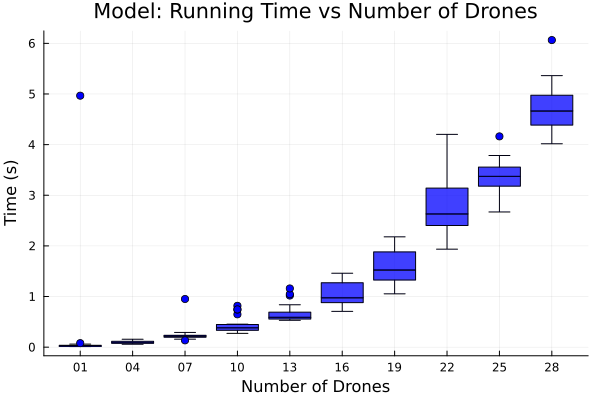
\includegraphics[width=0.8\textwidth]{img/julia_time_boxplot_vs_drones.png}
    \caption{Exact Model time. Source: The authors.}
    \label{fig:exact_model_time}
\end{figure}

\begin{figure}[H]
    \centering
    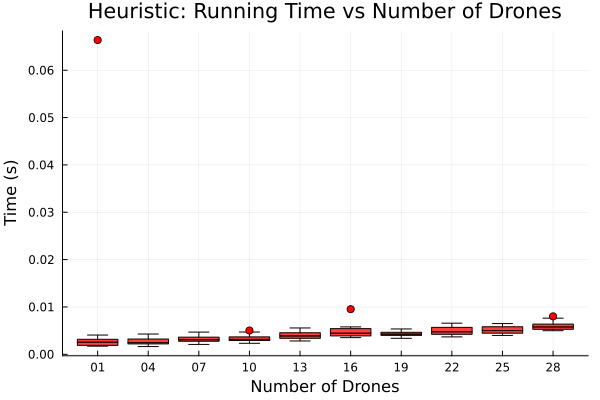
\includegraphics[width=0.8\textwidth]{img/cpp_time_boxplot_vs_drones.png}
    \caption{Heuristic time. Source: The authors.}
    \label{fig:heuristic_time}
\end{figure}

\subsection{Heuristic Behavior and Transition}
\label{sec:transition}

In this section, we propose an experimental setup to analyze the behavior of the heuristic in high-traffic configurations. We compare the heuristic's performance with the optimal distance for each drone in a collision-free environment, where the optimal path for each drone does not consider other drones in the grid (Manhattan distance).

Primarily, we define the optimal distance per drone as the Manhattan distance between its start and end points. For each drone $k \in \mathcal{R}$, with starting position $(x_k^{\text{start}}, y_k^{\text{start}})$ and ending position $(x_k^{\text{end}}, y_k^{\text{end}})$, the Manhattan distance $D_k$ is given by: \[
D_k = |x_k^{\text{start}} - x_k^{\text{end}}| + |y_k^{\text{start}} - y_k^{\text{end}}|\text{.}
\]

We then calculate the actual path length $P_k$ for each drone $k$ based on the heuristic path, and compute the optimality ratio $R_k$ as follows: \[
R_k = \frac{P_k}{D_k}\text{.}
\]

The optimality ratio provides a measure of how efficiently the heuristic performs compared to the ideal (collision-free) path.

The experiments were conducted using a $6 \times 6$ grid with the number of drones ranging from 1 to 99. For each number of drones, 30 points were sampled.

The visualization of the heuristic performance can be measured in several ways. For our purpose, we chose two metrics:

\begin{itemize}
    \item \textbf{Normalized Distance}: This metric shows the actual path length taken by each drone normalized by the Manhattan distance. It illustrates how the heuristic manages to find paths in high-traffic scenarios compared to the optimal path lengths.
\end{itemize}

\begin{figure}[H]
    \centering
    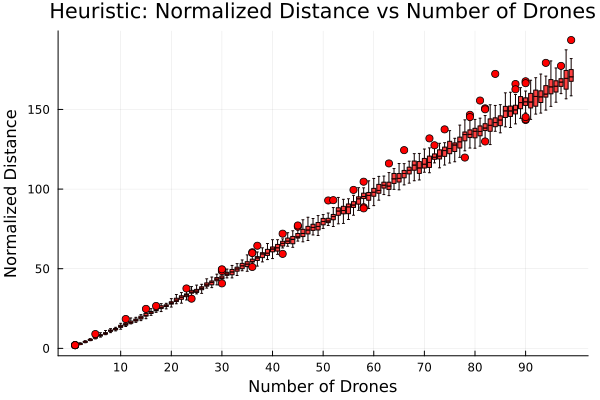
\includegraphics[width=0.8\textwidth]{img/cpp_normalized_distance_boxplot_vs_drones.png}
    \caption{Heuristic normalized distance per drone. Source: The authors.}
    \label{fig:heuristic_normalized_dist}
\end{figure}

Figure \ref{fig:heuristic_normalized_dist} displays the distribution of normalized distances for the heuristic, highlighting how the path lengths vary with an increasing number of drones. The box plot provides insights into the spread and central tendency of the heuristic's performance.

\begin{itemize}
    \item \textbf{Routing Time ($T$)}: This metric shows the time taken for the heuristic to compute the paths for all drones. It provides an understanding of the computational efficiency of the heuristic as the traffic increases.
\end{itemize}

\begin{figure}[H]
    \centering
    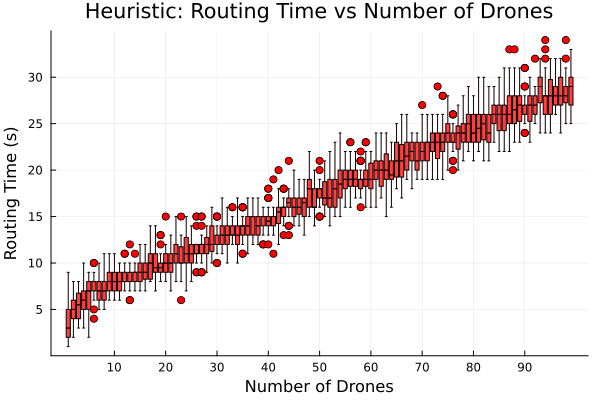
\includegraphics[width=0.8\textwidth]{img/cpp_routing_time_boxplot_vs_drones.png}
    \caption{Heuristic Routing Time ($T$) corresponding to Figure \ref{fig:heuristic_normalized_dist}. Source: The authors.}
    \label{fig:heuristic_normalized_routing_time}
\end{figure}

Figure \ref{fig:heuristic_normalized_routing_time} illustrates the routing times required by the heuristic as the number of drones increases. The box plot shows the variability in routing times and helps identify any trends or outliers. This result evinces the reasonability of the hybrid method in \ref{Hybrid_Methodology}, since we have a T that increases just linearly in the number of drones, even in a high traffic condition(36 cells available cells and 99 drones).

Together, these figures provide a comprehensive view of the heuristic's behavior under varying traffic conditions, demonstrating both its effectiveness in finding feasible paths and its computational efficiency. 